\documentclass[oneside,12pt]{report}  

% the dimensions of the page
\textheight=9.25in \topmargin=-0.5in   %See note in Chapter 8 of Sample Report about "Page scaling" option in Adobe
\textwidth=6.0in
\oddsidemargin=0.3in
\evensidemargin=0.3in  % Needed to balance even and odd pages in twoside print copy


% Useful packages
\usepackage{dtklogos}
\usepackage{amsmath}
\usepackage{bm}
%\usepackage[colorlinks=true,pagebackref,linkcolor=blue]{hyperref}
\usepackage{amsfonts}
\usepackage{amsthm}
\usepackage{amsmath}
\usepackage{algorithm}
\usepackage{algorithmic}
\usepackage{graphicx, subfigure}
\usepackage{caption}
\usepackage{excludeonly}

\usepackage{graphicx} 

%\usepackage{doc}
%% Following sets up logic and formatting for conditional twoside copying
%\usepackage{ifthen, color, fancyvrb}
%\usepackage{nextpage}\pagestyle{plain}
%\newcommand\myclearpage{\cleartooddpage
%  [\thispagestyle{empty}]
%  }

\DeclareMathOperator*{\argmin}{arg\ min}
\DeclareMathOperator*{\sign}{sign}

% Note special alternative codes for using TWO bibliographies; see cautionary note in
\DeclareGraphicsExtensions{ps,eps,PNG,png}

% Theorem-like command definitions:
\newtheorem{theorem}{Theorem}[chapter]
\newtheorem{lemma}{Lemma}[chapter]
\newtheorem{definition}{Definition}  % Note, this italicizes everything

% Print the chapter and sections in the toc
\setcounter{tocdepth}{1}

% Specify which files to typeset for this run (note that overall pagination is preserved)
%\includeonly{chapter1, chapter2}
% Specify which files NOT to typeset for this run (note that overall pagination is preserved)
%\excludeonly{}

% Groundwork for allowing double-sided copying with blank versos
\def\prefacesection#1{
\chapter*{#1}
\addcontentsline{toc}{chapter}{#1}
}

\begin{document}


\def\thefootnote{\fnsymbol{footnote}}

\thispagestyle{empty}

% The numbers below controls the amount of space between the following sections
\def\shiftdowna{0.32in}  % Adjust for balance
\def\shiftdownb{0.22in}  % Adjust for balance

% Set up the boiler plate at the top of the page

\begin{center}
\textbf{{\large Mathematical Modeling and Consulting }}\\

\vspace \shiftdowna

\includegraphics[width=0.5\textwidth]{jhu.png}\\

% Home Department
\vspace \shiftdowna
\underline {Sponsor}\\ 
\vspace{5pt}
\textbf{\large The RAND Corporation} \\
\vspace\shiftdowna
\textbf{{Progress Report}}

% TITLE
\vspace \shiftdowna
\textbf{{\Large Large Graphical Models to Explore the Effects of Globalization and Development on Prevalence of Obesity}}

% STUDENTS
\vspace{0.35in}
\underline {Team Members}\\

Michael Weinberger, \texttt{michael.lee.weinberger@gmail.com} \\
\vspace{3pt}
\text{Zhendan Zhu}, \texttt{zhendanzhu@hotmail.com} \\
\vspace{3pt}
\text{Shannon Cebron}, \texttt{scebron@cis.jhu.edu}

% INSTRUCTOR
\vspace \shiftdownb
\underline {Academic Mentor} \\
\vspace{5pt}
\text{Dr.~N.~.H.~Lee}, Applied Mathematics and Statistics\\
\texttt{nhlee@jhu.edu}

% Consultants
%\vspace \shiftdownb 
%\underline {Consultant}\\
%\vspace{5pt}
%Jason Bourne\\

% DATE
\vspace \shiftdowna
Date: Last Complied on \today

\end{center}

\vfill  %Fill page to force following note to bottom
\footnoterule
\noindent \small{This project was supported by Johns Hopkins University.}

% Begin ABSTRACT
\ifthenelse{\boolean{@twoside}}{\myclearpage}{}
\prefacesection{Abstract}

In recent years, obesity has become a global epidemic, affecting not only citizens of first-world countries, but also citizens of those countries experiencing rapid trade development. The link between globalization and obesity has been explored by some organizations, but not in a rigorous mathematical context. This project seeks to develop a mathematical description of this uptake in obesity, utilizing graphical constructs based in known information about countries’ development rates and trading habits, and using properties of these graphs to build regression models which can accurately predict obesity rates.

% Begin ACKNOWLEDGMENTS
%\ifthenelse{\boolean{@twoside}}{\myclearpage}{}
%\prefacesection{Acknowledgments}

% Table of contents, List of Figures, and List of Tables.
\ifthenelse{\boolean{@twoside}}{\myclearpage}{}
\tableofcontents

%\ifthenelse{\boolean{@twoside}}{\myclearpage}{}
%\listoffigures

%\ifthenelse{\boolean{@twoside}}{\myclearpage}{}
%\listoftables


\renewcommand{\thefootnote}{\arabic{footnote}}
\setcounter{footnote}{0}

\ifthenelse{\boolean{@twoside}}{\myclearpage}{}
%\include{A_Introduction}
%\include{B_TechnicalBackground}
%\include{C_ProblemStatement}
%\include{D_Analysis}
%\include{E_Results}
%\include{F_Conclusion}

%\include{chapter1}
%\include{chapter2}
%\include{chapter3}
%\include{chapter4}
%\include{chapter5}
%\include{chapter6}

\chapter{Introduction}

Obesity is a medical condition identified by a Body Mass Index (BMI) (an adjusted proportion between height and weight) greater than 30. Obesity is proven to have extreme effects on a person`s quality of life \cite{health}. It is a major predictor in several potentially deadly types of disease; a common cause of physical degradation in the body manifested through pain in the joints and difficulty walking and moving; an aggravator of existing conditions such as sleep apnea and acid reflux disease; and a known detriment to mental health for reasons of body image and self-confidence.

When present in large proportions in populations, obesity is a major public health problem and a leading cause of preventable death. Treatment for heart disease, asthma, and diabetes is costly, driving up the cost of health care for the whole population. Furthermore, lost work hours due to obesity-related health problems detract from the health of the local economy.

As of 2010, the United States Center for Disease Control reports that 35.7 percent of the American population is obese, and this number has been steadily increasing since the 1960s \cite{prevalence}. The federal government estimates that up to USD 117 billion is lost yearly due to direct and indirect costs of such an obese population \cite{prevalence}.

The prevalence of obesity is increasing in countries around the world, at the highest rates in countries recently achieving highly developed status as according to the Human Development Index (a weighted average exceeding 0.8 between measures of education, life expectancy, and personal wealth). However, in some countries this effect is more pronounced than in others, and at this level of detail, the spread of obesity is not well-understood. It is surmised that through increased trade and increased personal disposable income, more processed food has become available around the world. Furthermore, rapid changes in technology have allowed nations to become more culturally integrated with one another, and some experts suggest that citizens of developing countries are becoming more and more influenced by the dietary and exercise habits of their developed neighbors.

A better understanding of the interplay between development, globalization, and obesity may contribute positively to efforts to prevent the spread of this preventable, expensive, and deadly disease.

The RAND Corporation is a public policy thinktank which conducts research and analysis to support political decision-making and the public good. Many elected persons agree that legislation may help to curb the obesity epidemic, and it is important that this legislation is designed in an informed, rigorous manner. By working with the RAND Corporation to conduct this project, we can help to give lawmakers insight into what factors most prominently affect obesity trends.

\chapter{Technical Background}

Vast amounts of data for nations and sovereign entities are available from the CIA World Factbook and the World Health Organization's (WHO) databases. The data can be downloaded from these sources in .csv files. These .csv files can be imported into the R environment and merged so that a data frame is built with several different independent variables listed for each country. The CIA World Factbook and WHO refer to some countries by different names (e.g., the Republic of Korea is the same thing as South Korea). In order to merge the lists property despite these naming differences, another table was used which listed possible alternate names for each country, and this table was referenced during the merging process to ensure that South Korea and the Republic of Korea had their data combined. As a convention, in the data frame that was built, the name used by the CIA World Factbook tables is the country name listed in the data frame.


The R environment is effective for statistics and data management, but does not have a robust package for creating graphs. Python, however, does have such a feature. Therefore, the data from R must be converted into a .csv file again. However, individual data points for each country do not allow us to define the vertex-edge graphs that we would like to create. We also need data regarding the relationships between countries, such as bordering countries - this data will be used to define adjacencies in our graphs. This information is not available in a format that is as convenient. It must be mined from a webpage and processed to remove commas, footnotes, and other extraneous text that the CIA has included on the webpage. This was done in Microsoft Excel by pasting the contents of the webpage into a spreadsheet and processing the cells using Excel formulas. Then, the spreadsheet was also exported as a .csv file. Finally, the two .csv files will be imported into Python and used to create the graphs. This step has yet to be completed.


Python allows data to be extracted from graph objects, such as the neighborhood size for each vertex, shortest path data, or clique numbers. These data can also be arranged by country, and added back into the data frame as additional independent variables. After this step, we will have a long list of independent variables in the data frame. Using these variables as predictors, we can then start to build regression models using R's robust regression abilities. It is unlikely that a basic multiple linear regression model will fit the data well. We may need to experiment with other forms of regression, such as exponential or polynomial regression; furthermore, we may need to apply functions like logarithms to the predictor variables so that their relationship to the response variable (obesity rate) follows the assumptions of the model in question. This will be done on an ad-hoc basis based on diagnostics performed on the models, and at this time we cannot predict exactly what measures will be taken in order to build an effective regression model.

\chapter{Problem Statement}

Consider the following graph.

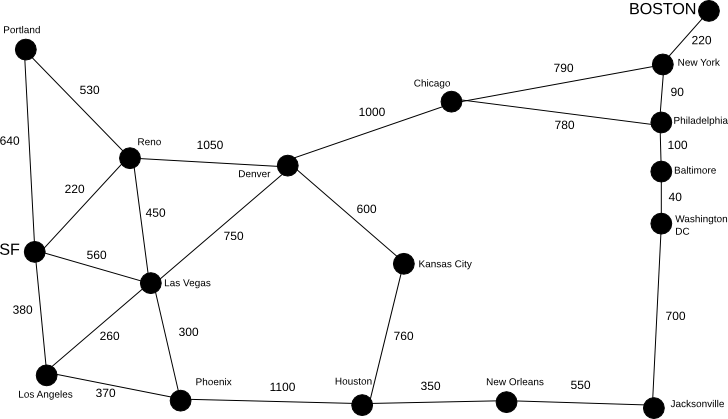
\includegraphics[width=\textwidth]{graph_map_of_us.png}\\

This graph was constructed using major US cities as vertices and the distance in miles between the cities as edge lengths. Though the vertices in our model will represent nations, not cities, this is one example of how the graph might be structured.

The problem with inferring information from the graph is choosing how to define adjacencies, edge lengths, and vertex weights; in addition,
it must be decided which graphical properties will then be examined in a statistical model. Our task is to use sequential regression modeling to
investigate which properties are important predictors of national obesity rates, and use this information to inform our graph definitions and our final statistical models.

\chapter{Analysis}

The proposed project consists of a few major components.

First, data needs to be acquired. A wealth of data is available from the CIA World Factbook, a reputable government-maintained website. Information can be
found on obesity rates, economic and trade data (such as GDP per capita, number of import/export partners, and income inequality), and national borders (numbers and names of bordering countries). This data will initially be handled in a data frame in either R or Python.

Secondly, the graphs need to be constructed. Both Python and Java offer fairly robust graphical structures and methods. Several different theoretical graphs will be created with a variety of definitions.

Thirdly, data will be extracted from the graphs. Measures such as neighborhood sizes, shortest paths, vertex degrees, and cliques and independent sets will be considered. This data will be tabulated and added to the original data frame.

Fourthly, a multiple linear regression model will be built to examine the appropriateness of a linear model for the data, as well as to give some initial insight into which variables are significant predictors of the national obesity rate. Predictor variables in this regression model will include items from the first step such as GDP per capita, and will also include items from the third step, e.g., number of developed countries within 1000 miles. The insights from this initial model will allow a more appropriate regression model to be designed, which may be non-linear or mixed in nature, depending on the results of the first model. This model will have a strong theoretical ability to predict the obesity rate in new countries not included in the original data, as well as give an effective account for the variation within the original data.

If time permits, then the graphical modeling stage will be revisited, with additional data considered, such as information about food market and international restaurant chain presence.

If data on past obesity rates is not readily available, then the project will be scaled down to exclude the model to predict future obesity rates, since for this model data is needed from more than one point in time. In this case, the current obesity rate model will be expanded to consider more data that otherwise would only have been included with time permitting.

\chapter{Progress}

Our work on the project so far has focused on data collection and processing (much of which is described in the technical background section of this report). Data for 190 countries has been collected, with obesity rates as well as 14 other independent variables. These independent variables are as follows:

\begin{enumerate}

\item GDP per capita

\item Percentage of children under the age of 5 who are underweight

\item Education expenditures as a percentage of GDP

\item Inflation rate

\item Gini index for families

\item Population growth rate

\item Number of total internet users

\item Health expenditures as a percentage of GDP

\item Birth rate

\item Total electricity consumption

\item Fertility rate

\item Unemployment rate for persons aged 18-24

\item Total population

\item Imports (in US dollars) per person

\end{enumerate}


Below is a snapshot of the data frame in RStudio (a front-end development environment for R).
\\

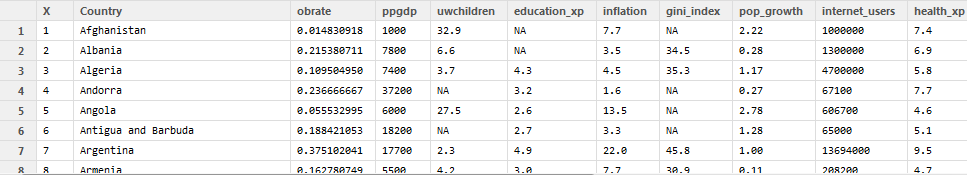
\includegraphics[width=\textwidth]{dataframe_snapshot.png}\\

In an exploratory multiple linear regression model, 6 of these independent variables were significant predictors of obesity rate (according to hypothesis tests on the estimated slope coefficients produced by R): GDP per capita; percentage of underweight children; number of internet users; electricity consumption; total population; and per person imports. The following is a graph of percentages of underweight children versus obesity rate, with a regression line plotted onto it. This relationship was highly statistically significant. Here is also displayed a snapshot of the multiple linear regression model with coefficients and significance markers.

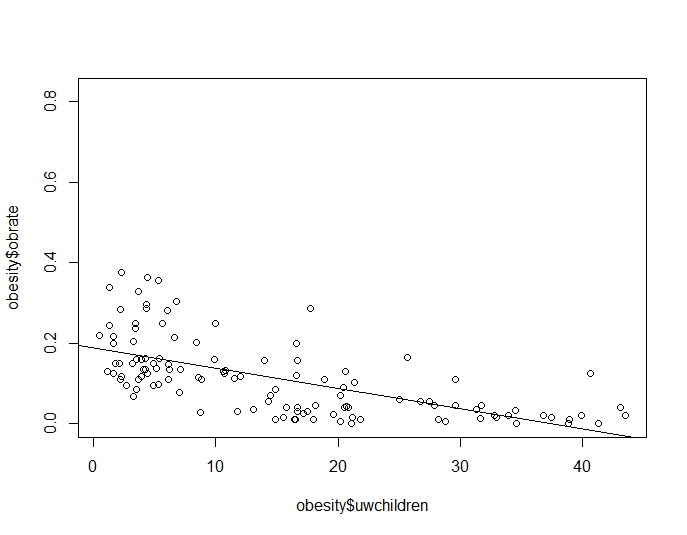
\includegraphics[width=\textwidth]{underweight_children.png}\\

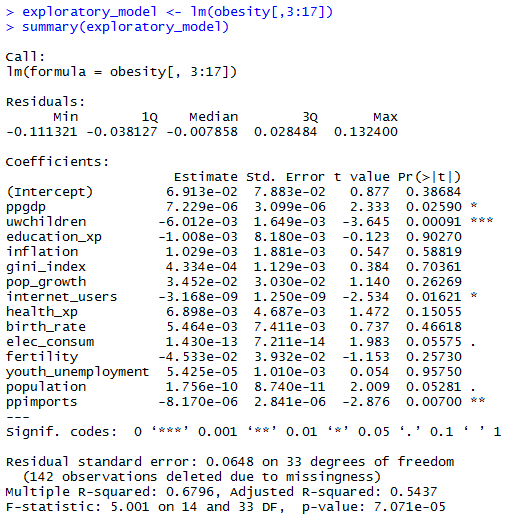
\includegraphics[width=.75\textwidth]{multi_regression.png}\\

We have also gathered formatted data of all geographic adjacencies between countries.


Going forward, we will start to build graphs in Python and explore ways to infer data from them. The 6 variables which were significant in the exploratory regression tests will be given higher consideration when building the graphs. For example, one piece of data we might consider is the sum of internet users of all of a country's geographical neighbors. There will be many ways to gain information from the graphs, and a lot of the work on this stage of the project will simply be experimenting with different details to find out which information is of interest.


After we have thoroughly perused the graphs in Python, the data we gain from them (e.g. number of neighboring internet users) will be added to the data frame in R, and we can continue with the regression process.

%\chapter{Conclusion}

\ifthenelse{\boolean{@twoside}}{\myclearpage}{}

\appendix
\ifthenelse{\boolean{@twoside}}{\myclearpage}{}

%\chapter{Lemmas}\label{Lemma}

\chapter{Glossary}\label{Glossary}

\vspace{12pt}

\vspace{8pt}
\noindent {\bf Obesity}. A medical condition that Body Mess Index is greater than 30.

\vspace{8pt}
\noindent {\bf Body Mess Index}. Body Mess Index is defined as the individual's body mass divided by the square of his or her height. .

\vspace{8pt}
\noindent {\bf Vertex-edge graph}. A set of vertices (also called nodes), along with a set of edges (also called arcs), in which each edge must correspond to two vertices as its endpoints. The edge may or may not have direction. A simple graph is one that does not allow multiple edges between the same two vertices, or an edge that has the same vertex as both of its endpoints.

\vspace{8pt}
\noindent {\bf Human Development Index}. A composite statistic of life expectancy, education, and income indices to rank countries into four tiers of human development.

\vspace{8pt} \noindent {\bf Vertex degree}. In graph theory, the degree (or valency) of a vertex of a graph is the number of edges incident to the vertex, with loops counted twice..

\vspace{8pt} \noindent {\bf Clique}. In graph theory, a clique is a subset of a graph's vertices such that every two vertices in the subset are connected by an edge.

\vspace{8pt} \noindent {\bf Regression}. Regression is a method for modeling the relationship between a single response variable and one or more independent variables which are thought to have a relationship with the response variable. If this relationship is linear, then it is linear regression. If the response variable comes from a finite set of outcomes, then we use logistic regression, which calculates the odds of the response variable taking on each outcome. Coefficients are estimated for each independent variable such that the deviation between actual and predicted values is minimized.

\vspace{8pt} \noindent {\bf Hypothesis test}. A hypothesis test compares a null hypothesis to an alternative hypothesis. The null hypothesis is rejected if, under the assumption that it is true, the probability of observing the true data is less than a specified significance value. In the statistics community it is standard to use 0.05 as this value.

\vspace{8pt} \noindent {\bf Gini index}. A probabalistic measure of dispersion of incomes in a society, where a higher Gini index indicates more income inequality - i.e., a bigger gap between rich and poor.


\ifthenelse{\boolean{@twoside}}{\myclearpage}{}
\chapter{Abbreviations}\label{Abbreviations}


\noindent CIA. Central Intelligience Agency
\vspace{5pt}

\noindent GDP Gross Domestic Production

\vspace{5pt}

\noindent BMI. Body Mass Index

\vspace{5pt}

\noindent WHO. World Health Organization

\vspace{5pt}

%\endinput

% Add your bibliography to Contents
\ifthenelse{\boolean{@twoside}}{\myclearpage}{\newpage}
\addtocontents {toc}{\protect \contentsline {chapter}{REFERENCES}{}}
\addcontentsline{toc}{chapter}{Selected Bibliography Including Cited Works}  

% Bibliography must come last.
\bibliographystyle{plain}
\renewcommand\bibname{Selected Bibliography Including Cited Works}
\nocite{*}  % List ALL references in your references, not just the ones cited in the text.
% This scheme automatically alphabetizes the Bibliography.
\bibliography{Biblio}
\end{document}
